% !TeX spellcheck = en_US
\addscenariosection{1}{Clash Scenario}{Secret Bomb Stash}{\images/secret-bomb-stash.png}

\begin{multicols}{2}

\textbf{Author:} NeuroN

\textbf{Source:} \href{https://discord.com/channels/740870068178649108/1278750250722525203/1278750250722525203}{Archon Studios Discord}

\textit{There are rumors of the abandoned bomb stash in this area.
Use it to destroy your opponents.
But be careful, because your enemies might be one step ahead of you.}

\subsection*{\MakeUppercase{Scenario Length}}
This Scenario is played over 8 Rounds, with possible 4 additional tie-breaking ones.

\subsection*{\MakeUppercase{Player Setup}}
\textbf{Player Count:} 2--4, 6 Player FFA or 2vs2, 2vs2vs2, 3vs3 Alliance

\textbf{Starting Resources:} 40 \svg{gold}

\textbf{Starting Income:} 20 \svg{gold}, 2 \svg{building_materials}, 1 \svg{valuables}

\textbf{Starting Units:}
\begin{itemize}
  \item a Few of two \svgunit{bronze} Units with the lowest Recruitment cost
  \item a Few \svgunit{silver} Units with the lowest Recruitment cost
\end{itemize}

\textbf{Town Buildings:} \svgunit{bronze} Dwelling, \svgunit{silver} Dwelling, Citadel, Mage Guild

\textbf{Map Tile Pool:} None

\textbf{Additional Bonus} (replaces regular Starting Bonus):

\begin{itemize}
  \item Search (4) the Artifact Deck and shuffle the Card into your M\&M Deck
\end{itemize}
Before the start of the Scenario instead of normal Search (2) Spells twice, each player performs Search (4) Spells once.
\textbf{Players start at Level III} (before the start of the Scenario instead of normal Search (2) Abilities twice, each player performs Search (4) Abilities once).

\subsection*{\MakeUppercase{Map Setup}}
\begin{itemize}
  \item Center (VI--VII) Map Tile \textbf{must} contain the Grail Field.
  \item Every near Tile must contain an Obelisk (if that's not possible, treat Witch Huts as Obelisks).
  \item Take the following Map Tiles and arrange them as shown in the Scenario map layout ($P$ stands for the number of players):
\end{itemize}

\textbf{For a 2- and 4-player Scenario:}
\begin{itemize}
  \item $\boldsymbol{P}$ × Starting (I) Map Tile
  \item 4 × Near (IV--V) Map Tile
  \item 1 × Center (VI--VII) Map Tile
\end{itemize}

\textbf{For a 3- and 6-player Scenario:}
\begin{itemize}
  \item $\boldsymbol{P}$ × Starting (I) Map Tile
  \item 6 × Near (IV--V) Map Tile
  \item 1 × Center (VI--VII) Map Tile
\end{itemize}

\subsection*{\MakeUppercase{Objective}}
Deposit bombs (Grail) into enemy Town.

\subsection*{\MakeUppercase{Defeat Conditions}}
Players loose if they don't score enough VPs in the designated amount of turns.

\subsection*{\MakeUppercase{Timed Events}}

\textbf{Every Astrologers Proclaim Round:}
\begin{itemize}
  \item Each Hero gains +1 \svgeven{movement}, except for the current bomb carrier.
\end{itemize}

\newpage

\subsection*{\MakeUppercase{Additional Rules}}

During this Scenario:

\begin{itemize}
  \item Heroes cannot attack other players' Towns without carrying the bomb.
  \item Heroes cannot attack bomb carrier from their Starting Town Field.
\end{itemize}

Center Tile:
\begin{itemize}
  \item On Center Tile, Player can freely move through the neutral battles Level VI, as if they had basic pathfinding effect (they can choose to fight there, but don't have to, and can't end turn there without resolving the battle).
  \item Level VII combat is ignored. The Hero that visits the Grail space gets the bomb(grail token). Put the Grail token under bomb carrying Hero's miniature.
\end{itemize}

Bomb:

\begin{itemize}
  \item Bomb carrier cannot gain extra \svgeven{movement} from any Card/Town Building/Map Location or any other effects.
  \item If your other Hero or allied Hero is adjacent to bomb carrier you can transfer the bomb to them.
  \item If defeated, the bomb is put on the space the Hero was defeated on, and can be claimed by any other Hero by visiting that Field.
  \item If held by main Hero:
  \begin{itemize}
    \item If defeated, the Hero does not have to pay their opponent gold, nor do they gain \svg{morale_negative}
  \end{itemize}
  \item If held by a Secondary Hero:
  \begin{itemize}
    \item If defeated, the Hero is moved to Town instead of being removed.
    \item The Hero can use M\&M Deck during battle.
  \end{itemize}
\end{itemize}

Obelisks:
\begin{itemize}
  \item When first flagged, that Hero gains +1 \svgeven{movement}
  \item On each visit (including first) player can choose to either:
  \begin{itemize}
    \item Move the visiting Hero to any other Obelisk already flagged by you (if said Obelisk is occupied by another Hero, your Hero cannot move there).
    \item If the Hero carries the bomb, transfer the bomb to your other Hero (or any of the allied Heroes).
  \end{itemize}
\end{itemize}

\end{multicols}

\begin{tikzpicture}[overlay]
  \centering
  \node at (4.5, -4) {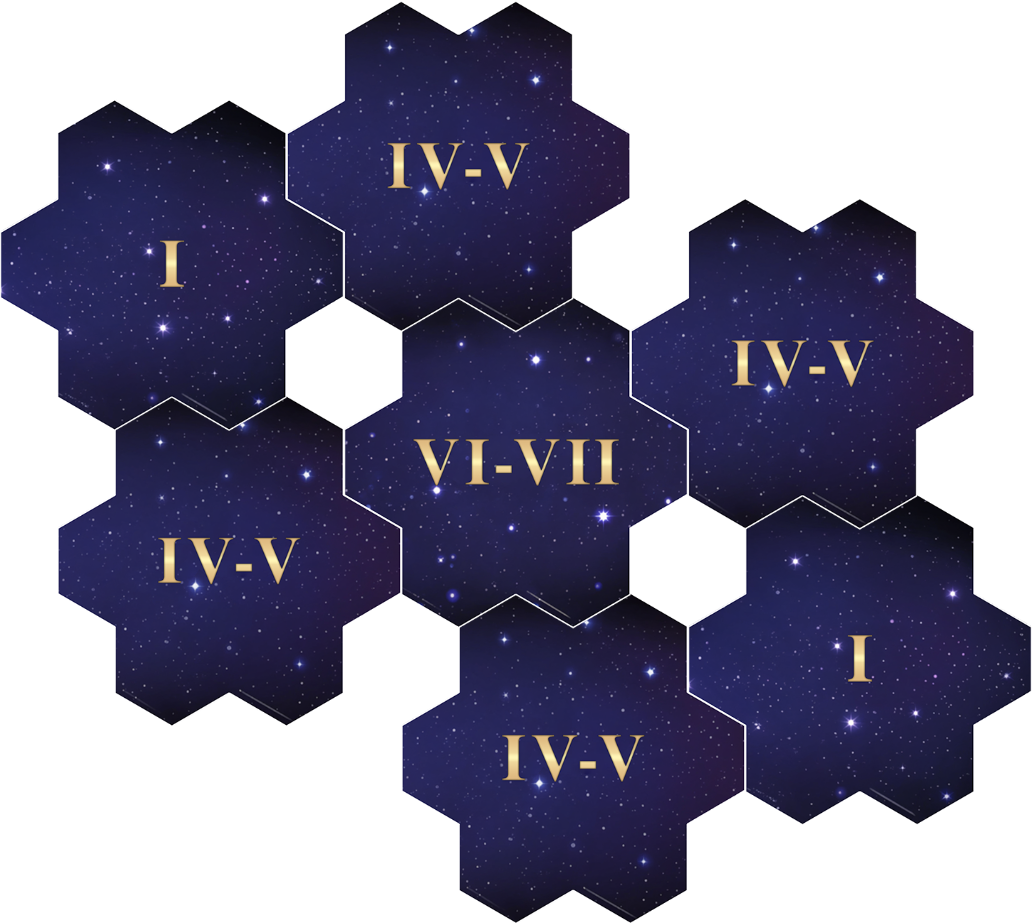
\includegraphics[scale=0.2]{\maps/secret-bomb-stash-2p.png}};
  \node at (4.5, -8) {\footnotesize{\textbf{\MakeUppercase{2-PLAYER SCENARIO}}}};
  \node at (14, -4) {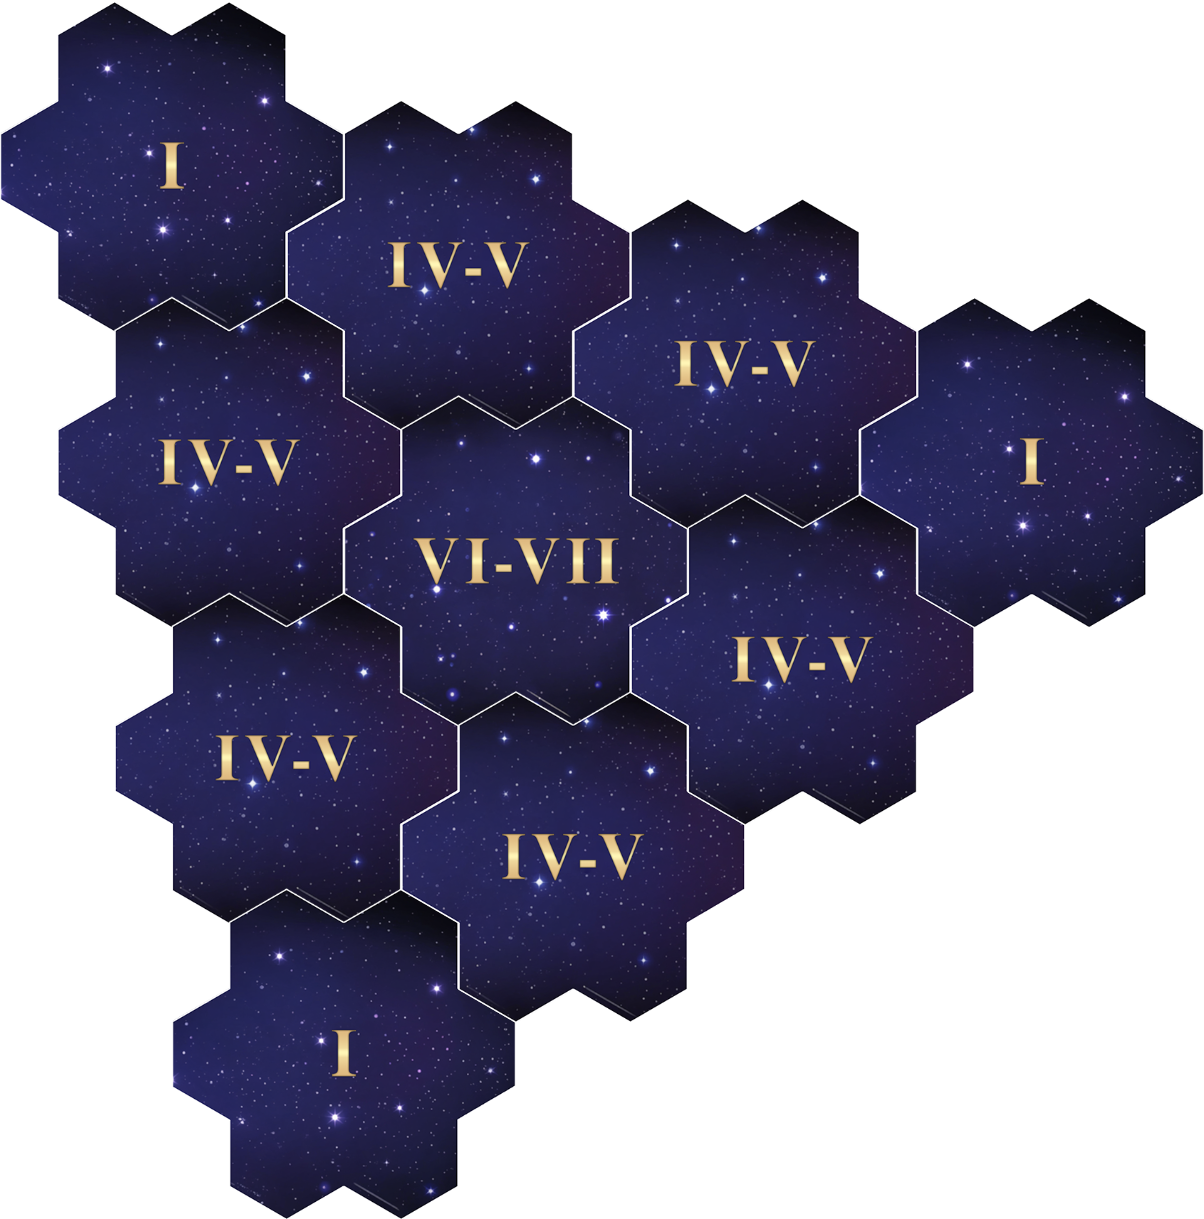
\includegraphics[scale=0.2]{\maps/secret-bomb-stash-3p.png}};
  \node at (14, -9) {\footnotesize{\textbf{\MakeUppercase{3-PLAYER SCENARIO}}}};
\end{tikzpicture}

\newpage

\begin{tikzpicture}[overlay]
  \centering
  \node at (4.5, -5) {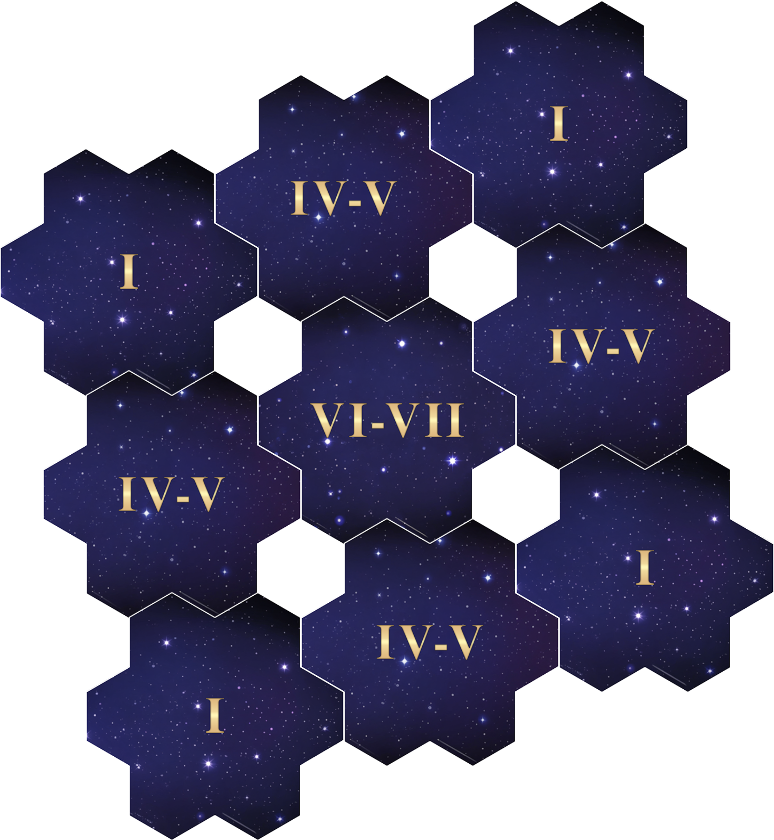
\includegraphics[scale=0.25]{\maps/secret-bomb-stash-4p.png}};
  \node at (6, -10) {\footnotesize{\textbf{\MakeUppercase{4-PLAYER SCENARIO}}}};
  \node at (12.1, -16.5) {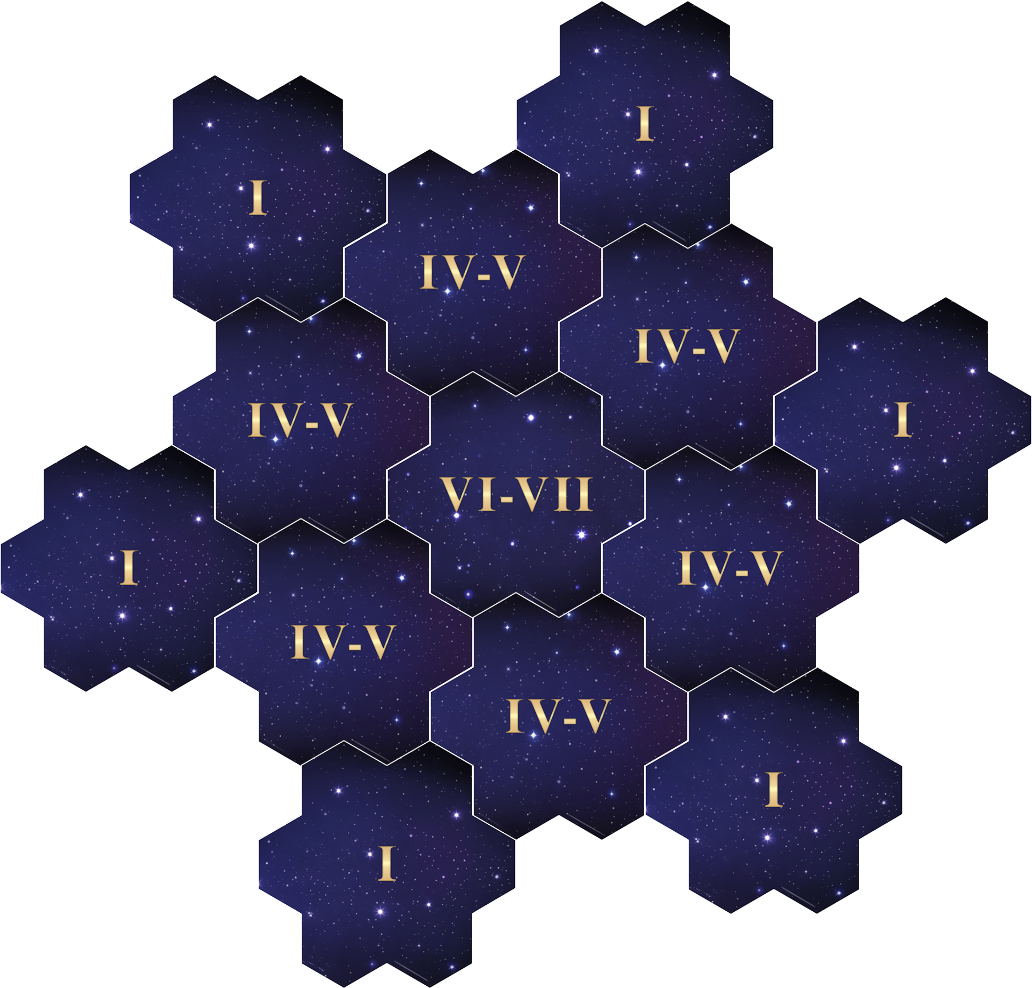
\includegraphics[scale=0.25]{\maps/secret-bomb-stash-6p.png}};
  \node at (12.1, -23) {\footnotesize{\textbf{\MakeUppercase{6-PLAYER SCENARIO}}}};
\end{tikzpicture}
